\providecommand{\main}{../../../..}
\documentclass[\main/dresen_thesis.tex]{subfiles}

\begin{document}
  \paragraphNewLine{Scanning Electron Microscopy}
    % The spin-coated nanospheres on silicon substrate are qualitatively viewed by SEM micrographs measured with a Neon Zeiss 40 (\refsec{ch:instruments:laboratoryInstruments:sem}).
    % To obtain cross-sectional views, a piece of a sample is cut on two opposing sides with a diamond cutter and then subsequently broken downward to obtain a clean breaking line, from which SEM measurements can be performed.
    % The micrographs are measured at $5 \unit{kV}$ and the images from the backscattering electrons are shown to obtain a strong contrast.

  \paragraphNewLine{Grazing-Incidence Small-Angle X-ray Scattering}
    % All spin-coated samples were measured at the beam line BM26B \refsec{ch:lss:BM26B} in the ESRF at a wavelength of $\lambda \eq 1.03 \unit{\angstrom}$.
    % For each sample a measurement was performed at a large sample-to-detector distance of $6.54 \unit{m}$ and at a shorter sample-to-detector distance of $2.90 \unit{m}$.
    % The collimation slit is set to $0.3 \times 0.5 \unit{mm^2}$ for each measurement, and every sample is evaluated at an incident angle of $0.2 \unit{^\circ}$.

    % For both samples, a strip of $0.02 \nm^{-1}$ width along the Yoneda band is integrated and compared to the form factor obtained by small-angle X-ray scattering.
    % The scattered intensity for the nanostructure along the Yoneda band is calculated as product of a structure factor and the form factor
    % \begin{align}
    %   I(q) \eq I_0 S(q) |P(q)|^2 + I_\mathrm{bg},
    % \end{align}
    % where $I_0$ is a scaling factor and $I_\mathrm{bg}$ is a incoherent noise background that is not directly associated with the scattering from the nanoparticles.
    % The used form factor $|P(q)|^2$ is hereby given by using the best fit of the nanoparticles from SAXS as determined in \refsec{sec:looselyPackedNS:nanoparticle:sas}.
    % As no calibration measurement has been performed at BM26B, the data is given in the arbitrary count units of the detector.
    % The structure factor for hard spheres of radius $R_\mathrm{HS}$ and with a packing fraction $\eta$ can be calculated analytically in the Percus-Yervick approximation \cite{Percus_1958_Analy, Wertheim_1963_Exact, Pedersen_1997_Analy} and is given by
    % \begin{align}
    %   S(q) &\eq \frac{1}{1 + 24 \eta \frac{G(2 q R_\mathrm{HS})}{2 q R_\mathrm{HS}} }
    % \end{align}
    % with
    % \begin{align}
    %   \begin{split}
    %     G(x)   &\eq \frac{(1 + 2\eta )^2}{(1 - \eta )^4} \cdot \frac{ \sin(x) - x \cos(x)}{x^2}\\
    %            & + \frac {-6 \eta (1 + \eta / 2)^2}{(1 - \eta )^4} \cdot \frac{2 x sin(x) + (2 - x^2) \cos(x) - 2}{x^3}\\
    %            & + \frac{\eta (1 + 2\eta )^2}{2(1 - \eta )^4} \cdot \frac{-x^4 \cos(x) + 4 [(3 x^2 - 6) \cos(x) +(x^3 - 6 x) \sin(x) + 6]}{x^5}\\
    %   \end{split}
    % \end{align}

  \paragraphNewLine{X-Ray Reflectometry}
    % XRR was performed on both SC-IOS-11 and SC-IOS-7 using a Bruker D8 Advanced at the \textsc{Forschungszentrum J\"ulich} \refsec{ch:instruments:laboratoryInstruments:xrr}.
    % The X-ray reflectometer was equipped with a Cu-K$\alpha$ source ($\lambda \eq 1.54 \unit{\angstrom}$) and a $q$-range of $0 \ldots 0.15 \unit{\angstrom^{-1}}$ is evaluated by measuring $2 \theta \eq 0 \ldots 1 \unit{^\circ}$ in $0.005 \unit{^\circ}$ steps over an integrated time of approximately $1 \unit{h}$.
    % The collimation slit on the instrument is $0.2 \unit{mm}$ and both samples have a width of approximately $20 \unit{mm}$.

    % To evaluate the reflectivity, a footprint correction is performed as described in \refsec{ch:methods:xrr}, assuming a equidistributed beam profile.
    % As substrate, the scattering length density of silicon is fixed to the literature value at the given wavelength ($\rho_\mathrm{Si} \eq 20.062 \cdot \unit{10^{-5} \angstrom^{-2}}$) and a spacer layer is allowed for the case of a thin \ch{SiO2} or any organic residues in between silicon and the nanospheres.

    % \begin{figure}[!htbp]
    %   \centering
    %   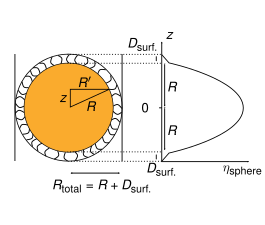
\includegraphics{looselyPackedNP_sphereProfile}
    %   \caption{\label{fig:looselyPackedNP:layerCharacterization:sphereProfile}Evaluation of the cross-section area fraction in comparison to a surrounding cylinder with respect to the height for a sphere with a core radius of $R$ and a oleic acid shell of thickness $D_\mathrm{OA}$.}
    % \end{figure}
    % To model a nanosphere layer, the area fraction of the spheres is needed.
    % The cross-sectional area fraction for a single sphere is given by a parabola, which is trivially derived using the Pythagorean theorem.
    % For a sphere with a surfactant shell, \reffig{fig:looselyPackedNP:layerCharacterization:sphereProfile} can be used to determine the area fraction of the core $\eta_\mathrm{core}$ and the shell $\eta_\mathrm{shell}$, which when evaluated with respect to a surrounding cylinder of radius $R + D_\mathrm{OA}$ are given by
    % \begin{align}
    %   \eta_\mathrm{core} (z)
    %             &\eq \begin{cases}
    %             \eta \frac{R^{2} - z^2}{(R+D_\mathrm{OA})^2}, &\mathrm{for\,}|z|<R \\
    %             0,                                            &\mathrm{else}
    %             \end{cases}\\
    %   \eta_\mathrm{shell} (z)
    %     &\eq \begin{cases}
    %       \eta \frac{2 R D_\mathrm{OA} + D_\mathrm{OA}^2}{(R+D_\mathrm{OA})^2}, &\mathrm{for\,}|z|<R \\
    %       \eta \frac{(R + D_\mathrm{OA})^2 - z^2}{(R+D_\mathrm{OA})^2}, &\mathrm{for\,}R<|z|<R+D_\mathrm{OA} \\
    %       0,                                            &\mathrm{else}
    %     \end{cases}
    % \end{align}
    % where $\eta$ is then the two-dimensional packing density of the surrounding cylinder in the layer.
    % The scattering length density profile $\rho(z)$ of a layer of nanospheres in a matrix of scattering length density $\rho_\mathrm{matrix}$ is then given by
    % \begin{align}
    %   \label{eq:looselyPackedNP:layerCharacterization:sldFromAreaFraction}
    %   \rho(z) \eq \rho_\mathrm{matrix} + (\rho_\mathrm{core} - \rho_\mathrm{matrix}) \eta_\mathrm{core}(z) + (\rho_\mathrm{shell} - \rho_\mathrm{matrix}) \eta_\mathrm{shell}(z),
    % \end{align}
    % where $\rho_\mathrm{core}$ and $\rho_\mathrm{shell}$ are the respective scattering length densities of the core and the shell.

    % This formulation can easily be extended to overlapping nanosphere layers by calculating the sum of the respective area fractions for each layer before determining the SLD by \refeq{eq:looselyPackedNP:layerCharacterization:sldFromAreaFraction}.
    % This procedure is performed for both SC-IOS-11 and SC-IOS-7, where as initial model a stack of nanospheres is given, where each layer is pitched on the vertical axis by $\sqrt{8/3} (R + D_\mathrm{OA})$, which would be the distance of two sphere centers for an ideal close sphere packing.
    % The model is fitted by varying the layer density $\eta$ and a shift from the ideal pitch $\Delta z$ for each layer respectively.
    % The parameters for the nanosphere size, surfactant thickness and scattering length density are used as obtained from SAS, noting that the SLD are readjusted for the different X-ray wavelength at the reflectometer with respect to the small-angle scattering experiments.
    % As roughness model a linearly increasing roughness $\sigma \eq \sigma_0 + \Delta \sigma z$ is used to describe a possibly increasing roughness with stack height.


  \paragraphNewLine{Polarized Neutron Reflectometry}
    The three colloidal crystals, CC-Fe-0.25, CC-Fe-0.37 and CC-Fe-0.50 were characterized on the polarized neutron reflectometer MARIA at MLZ.
    The neutron wavelength was selected to $5 \unit{\angstrom}$ and a wavelength spread of $10 \unit{\%}$ (FWHM) is given by the instrumental scientists.
    The collimation and sample slits along the scattering direction are set to $2 \unit{mm}$, the collimation-to-sample distance was $4.1 \unit{m}$ and the sample-to-detector distance was $2.093 \unit{m}$.
    Each sample was measured at a temperature of $10 \unit{K}$ after cooling in near zero field ($0.9 \unit{mT}$ guide field), subsequent at a saturating field of $1.08 \unit{T}$ and again in remanence at guide field.
    After that, each sample was warmed to $250 \unit{K}$, sufficiently above the blocking temperature, and then cooled back to $10 \unit{K}$ while applying the saturating field.
    After field-cooling, the sample was then measured once more in saturation and remanence, which totals in five neutron reflectometry measurements for each sample at $10 \unit{K}$.
    For each case, the reflectivity $R^{+}$, for neutrons polarized parallel to the magnetic field direction, and the reflectivity $R^{-}$, for neutrons that are polarized anti-parallel to it, is measured.
    No polarization analysis is performed for the sake of having higher counting statistics in the two channels.

    For the measurements, the incident angle was increased up to $6 ^\circ$, where the angle step is increased for three ranges.
    The first range up to $1 ^\circ$ has a step of $0.02 ^\circ$ is set.
    For a second range from $0.8 ^\circ$ up to $3.5 ^\circ$ a step of $0.05 ^\circ$ is chosen and for the last range from $2.8 ^\circ$ up to $6 ^\circ$ a step of $0.2 ^\circ$ is set.
    The three ranges overlap intentionally such that they can be stitch together in case the scaling of the data to the monitor would show a disagreement, which was not the case in the executed experiments.
    At the first range, each point is measured for $30 \unit{s}$, whereas for the second $120 \unit{s}$ and the third range $135 \unit{s}$ are set due to the lower scattering intensity and to to obtain better statistics.

    For the data reduction, each detector image is corrected for the detector sensitivity and integrated along the dimension with relaxed collimation. 
    By this integration the data is given as a map of the scattered intensity with respect to the detector pixel $x$ along the scattering direction and with respect to the incident angle $\alpha_i$.
    This map is transformed and rotated to ($\alpha_i - \alpha_o$, $\alpha_i+\alpha_o$) coordinates by calculating $\alpha_o$ from
    \begin{align}
      \alpha_o = \alpha_i + \arctan \biggl( \frac{x - x_\mathrm{spec}}{L_\mathrm{SDD}} \biggr),
    \end{align}
    where $L_\mathrm{SDD}$ is the sample-to-detector distance and $x_\mathrm{spec}$ the center pixel where the specular beam is hitting.
    For the transformation and rotation, the data needs to be rebinned in the new coordinate system.
    To avoid the loss of resolution, a pixel-splitting algorithm is used for the rebinning, which is described in \refapp{ch:appendix:numericalMethods:rebinningPixelSplitting}.

    The specular intensity is obtained, by integrating on the transformed data a strip of $0.1 ^\circ$ width around the specular position on the intensity beam.
    The data is further corrected for the diffuse scattering by additionally integrating strips of $0.1 ^\circ$ width in the off-specular region from $\pm (0.1 ^\circ \ldots 0.2)$, which are subtracted from the specular intensity after being rescaled to adjust for a different numbers of contributing bins.

    Finally a footprint correction if performed for the data, where a equidistributed intensity of the beam is assumed.
    Using the mean intensity of $R^{+}$ below the critical angle, the data is rescaled to have the plateau on unity.
    The curve of $R^{-}$ is rescaled using the same factor, to avoid the introduction of systematic errors by using two different scaling factors.


  \paragraphNewLine{Vibrating Sample Magnetometry}
    % Yip

\end{document}